\section{Ứng dụng Data Warehouse và BI vào bài toán}
\subsection{Giới thiệu bài toán}
\subsubsection{Đặt vấn đề}
\textbf{Tổng quan về Health care: }\\
Health care hay chăm sóc sức khỏe là sự cải thiện sức khỏe thông qua phòng ngừa, chuẩn đoán, điều trị, cải thiện hoặc chữa bệnh, chấn thương và suy giảm thể chất và tinh thần khác ở người bệnh.\\

\textbf{Tổng quan về ảnh hưởng của thuốc lá đến phổi: }\\
Thuốc lá là nguyên nhân gây ra nhiều bệnh như: viêm họng, viêm phế quản, viêm phế quản phổi, bệnh phổi tắc nghẽn mạn tính, hen, ung thư phổi, ...\\
Bệnh phổi tắc nghẽn mạn tính là chỉ những tổn thương ở phổi có liên quan đến sự tắc nghẽn đường thở không phục hồi hoàn toàn. Mối liên quan giữa bệnh phổi tắc nghẽn mạn tính và hút thuốc cũng mạnh như với ung thư phổi.
Thuốc lá là nguyên nhân quan trọng nhất gây ra bệnh phổi tắc nghẽn mạn tính, có khoảng 15\% những người hút thuốc lá sẽ có triệu chứng lâm sàng của bệnh phổi tắc nghẽn mạn tính và 80 - 90\% người mắc bệnh phổi tắc nghẽn mạn tính là nghiện thuốc lá.\\
Ở hầu hết các nước, thuốc lá là nguyên nhân gây ra hơn 90\% ca tử vong vì ung thư phổi. Trung bình người hút thuốc làm tăng nguy cơ bị ung thư phổi lên từ 5 đến 10 lần so với người không hút thuốc.\\

\textbf{Lợi ích của kho dữ liệu đối với chăm sóc sức khỏe}
\begin{itemize}[label=$-$]
\item Báo cáo hiệu quả.
\item Quyết định lâm sàng tốt hơn.
\item Yêu cầu và thanh toán bảo hiểm được tối ưu hóa.
\item Cải thiện kinh nghiệm và kết quả của bệnh nhân.
\item Chăm sóc dựa trên giá trị được cá nhân hóa.
\item Lập kế hoạch chiến lược nâng cao.
\end{itemize}
\newpage
\subsubsection{Quy trình nghiệp vụ}
\begin{center}
            \begin{figure}[!h]
                \centering
                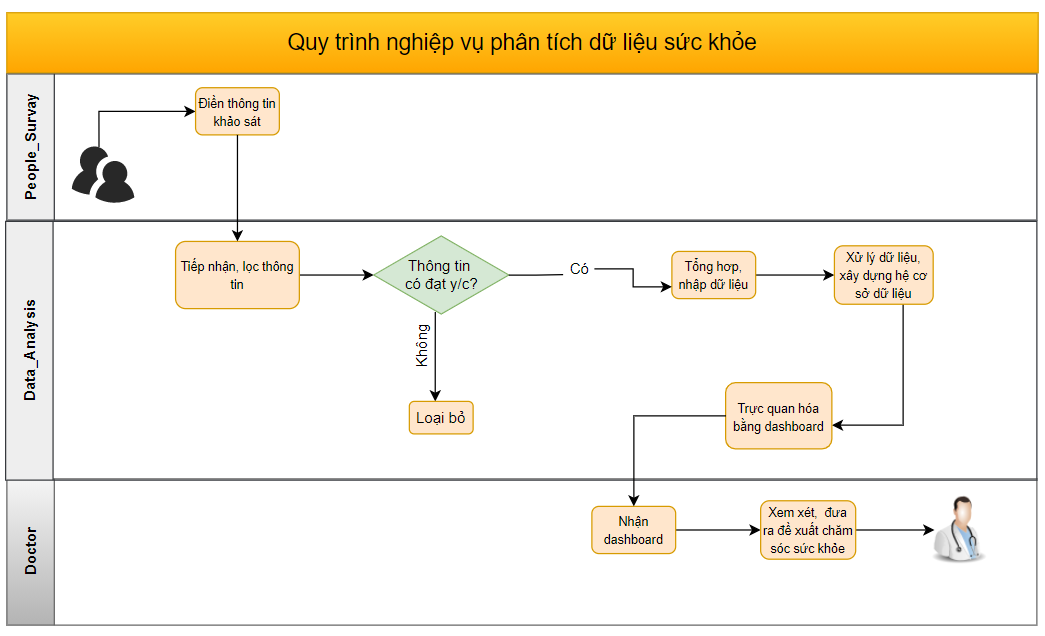
\includegraphics[scale = 0.6]{figures/Duyen/Phân tích nghiệp vụ.PNG}
              \caption{Quy trình nghiệp vụ}
            \end{figure}
\end{center}
%\newpage
\textbf{Quy trình xử lý}
\begin{itemize}[label=$-$]
    \item Đầu tiên, mọi người điền thông tin khảo sát.
    \item Sau đó, Data analysis sẽ tiến hành tiếp nhận và lọc thông tin, những thông tin không đạt yêu cầu sẽ bị loại bỏ ( Ví dụ những bản điền của người nào thiếu thông tin, thông tin điền không đúng ...), còn những thông tin đạt yêu cầu sẽ được tổng hợp, và xây dựng thành 1 bộ dữ liệu.
    \item Data analysis trực quan hóa bộ dữ liệu bằng dashboard và chuyển dashboard đến bác sĩ.
    \item Bác sĩ nhận dashboard, dựa vào đó để đưa ra những xem xét và đánh giá tình hình cũng như cách cải thiện sức khỏe của từng bệnh nhân.
\end{itemize}
\subsubsection{Quy mô dữ liệu}
Giới thiệu về bộ dữ liệu thì được chúng em lấy từ hệ thống giám sát yếu tố rủi ro hành vi là hệ thống điều tra qua điện thoại liên quan đến sức khỏe hàng đầu của quốc gia BRFSS.\\
Mục tiêu của hệ thống BRFSS: Thu thập dữ liệu tiểu bang về cư dân Hoa Kỳ về các hành vi nguy cơ liên quan đến sức khỏe, tình trạng sức khỏe mãn tính và việc sử dụng các dịch vụ phòng ngừa.\\
Kích thước bộ dữ liệu:
\begin{itemize}[label=$-$]
\newpage
    \item Dữ liệu gồm:
    \begin{itemize}[label=$+$]
        \item 3 file dữ liệu tương ứng với từng năm 2013 - 2015        \item Mỗi file chứa 1.5 triệu bản ghi.
    \end{itemize}
    \item Dữ liệu chủ yếu là dạng có cấu trúc
    \begin{itemize}
    \item Kích thước: 114MB
    \end{itemize}
    \item Chọn phân tích:
    \begin{itemize}[label=$+$]
        \item Dữ liệu khảo sát tại 6 tiểu bang: Alaska, California, Massachusetts, New York, Texas, Washington.
        \item 26 cột dữ liệu liên quan đến đối tượng khảo sát và vấn đề bệnh phổi mãn tính.
    \end{itemize}
\end{itemize}
%\newpage
\textbf{Mô tả 1 số trường dữ liệu quan trọng}
\begin{center}
            \begin{figure}[!h]
                \centering
                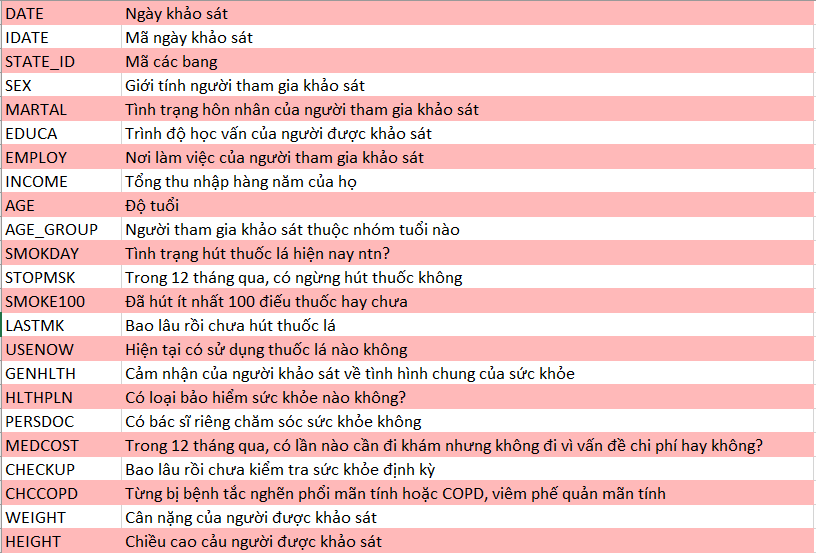
\includegraphics[scale = 1]{figures/Duyen/Mô tả 1 số trường dữ liệu quan trọng.PNG}
              \caption{Quy trình nghiệp vụ}
            \end{figure}
\end{center}
\subsubsection {Requirements}
\begin{itemize}
    \item \textbf{Input:} Dữ liệu khảo sát về ảnh hưởng của thuốc lá đối với phổi trong năm 2013 – 2015.
\item \textbf{Output: } Dashboard trả lời những câu hỏi:
\begin{enumerate}
    \item Phân tích và khảo sát thông tin người tham gia khảo sát:
    \begin{itemize}[label=$-$]
        \item Giới tính
        \item Độ tuổi
        \item Công việc
        \item Tình trạng hôn nhân
        \item Học vấn
        \item ...
    \end{itemize}
\item Phân tích và khảo sát tình trạng sức khỏe và khả năng tiếp cận y tế: 
    \begin{itemize}[label=$-$]
           \item  Tình trạng sức khỏe
            \item Có bảo hiểm y tế không?
            \item Có từng mắc bệnh phổi mãn tính không?
            \item Bao lâu chưa đi khám sức khỏe?    
            \item ...
        \end{itemize}
\item Phân tích và khảo sát thực trạng của việc hút thuốc lá:
    \begin{itemize}[label=$-$]
        \item Có hút thuốc lá không?
        \item Tần suất sử dụng thuốc lá?
        \item Đã từng hút ít nhất 100 điếu thuốc chưa?
        \item Đã từng có ý định bỏ thuốc lá chưa?
        \item ...
    \end{itemize}

\end{enumerate}
\end{itemize}



